\documentclass[conference]{IEEEtran}
\IEEEoverridecommandlockouts
\usepackage{cite}
\usepackage{amsmath,amssymb,amsfonts}
\usepackage{graphicx}
\usepackage{textcomp}
\usepackage{xcolor}

\def\BibTeX{{\rm B\kern-.05em{\sc i\kern-.025em b}\kern-.08em
    T\kern-.1667em\lower.7ex\hbox{E}\kern-.125emX}}

\title{
\vspace{1cm}
{
\includegraphics[width=0.15\textwidth]{/storage/emulated/0/FWC1/arm/IMG-20241021-WA0004.jpg       } \\ Arm Assignment} }

\author{Sivva Pranaykumar \\ Roll No: FWC22273 \\ sivvapranay.s@gmail.com}

\begin{document}
\maketitle

\section{ABSTRACT}
This project simplifies the Boolean function $F(A,B,C,D)=\sum m(0,2,5,7,8,10,12,13,14,15)$ using a Karnaugh Map (K-map). By identifying the essential prime implicants, the function is reduced to $BD$, $\overline{BD}$, and $AB$. These terms represent the minimal form of the function, efficiently expressing its logic.

\begin{figure}[h]
\centering
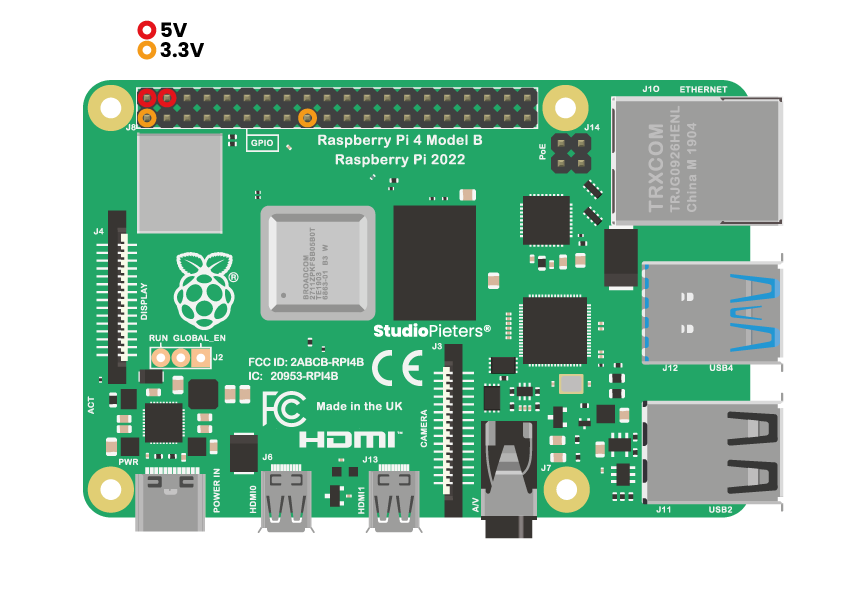
\includegraphics[width=0.35\textwidth]{/storage/emulated/0/FWC1/arm/17313068981125684858793623388663.png}
\caption{\label{fig:Gates}}
\end{figure}
\begin {figure} [h]
 \centering
 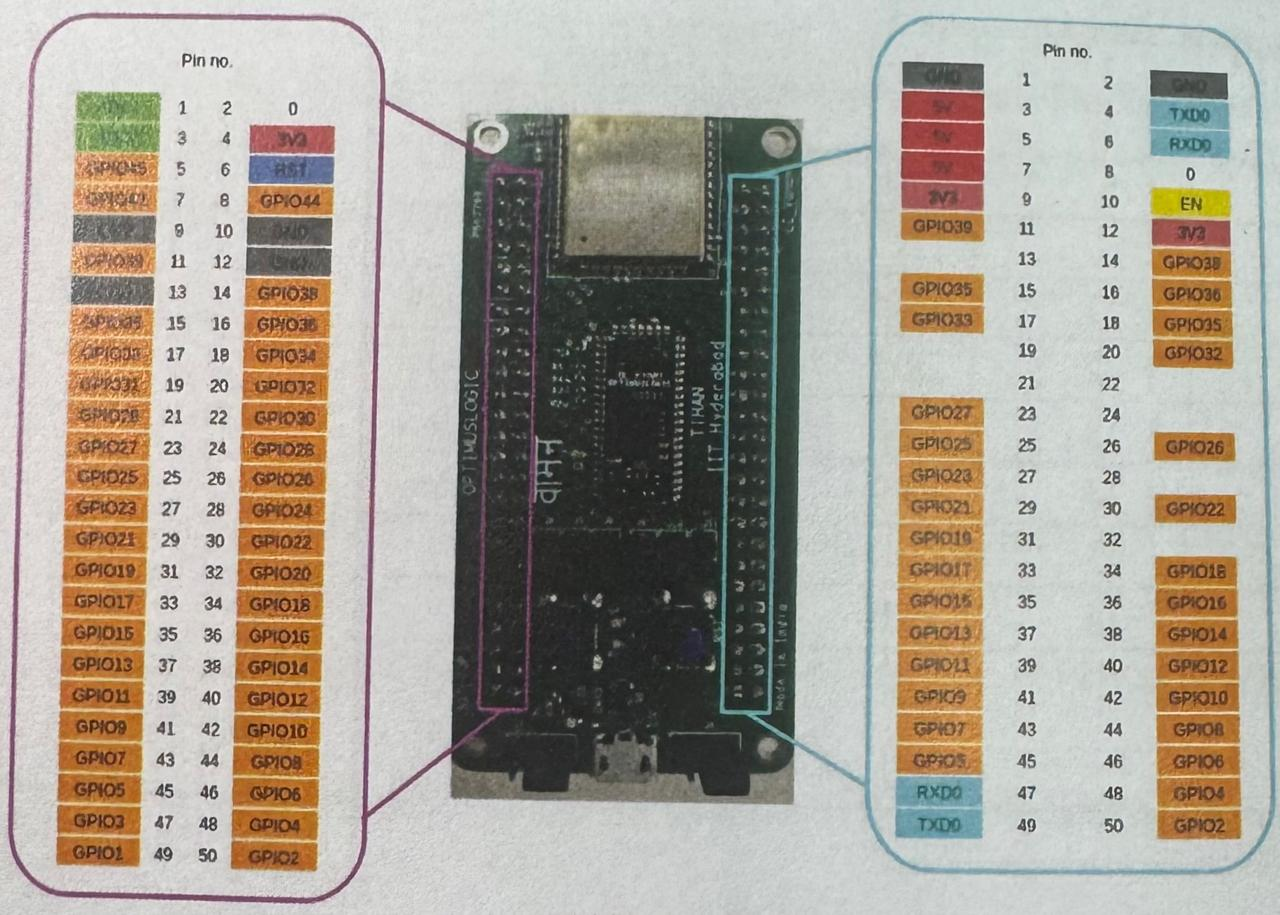
\includegraphics[width=0.35\textwidth]{  /storage/emulated/0/FWC1/arm/IMG-20241024-WA0005.jpg   }
 \caption{\label{fig:Gates}}
 \end {figure}




\section{COMPONENTS}
The required components list is given in Table I.

\begin{table}[htbp]
\centering
\begin{tabular}{|c|c|c|} \hline
Components & Value & Quantity \\ \hline
Vaman & & 1 \\ \hline
Raspberry Pi & & 1 \\ \hline
LEDs & & 3 \\ \hline
Jumper Wires & & 20 \\ \hline
Breadboard & & 1 \\ \hline
SD card & & 1\\
\hline
\end{tabular}
\vspace{0.1cm}
\caption{\label{tab:widgets}}
\end{table}

\section{PROCEDURE}
In this project, three LEDs were connected to the Vaman FPGA board to represent the essential prime implicants $BD$, $\overline{BD}$, and $AB$ of a Boolean function. GPIO pins were configured as outputs for the LEDs and inputs for the Boolean variables A, B, and D. The inputs A, B, and D were manually set by connecting the respective pins to either VCC or GND according to the truth table as shown in Table II. The logic for each prime implicant was implemented in code, where LEDs turned on or off based on the state of the inputs.

\begin{table}[htbp]
\centering
\begin{tabular}{|c|c|}
\hline
Vaman Board & LED \\ \hline
GPIO\_PIN\_9 & LED\_1 \\ \hline
GPIO\_PIN\_10 & LED\_2 \\ \hline
GPIO\_PIN\_11 & LED\_3 \\ \hline
GPIO\_PIN\_2 & Gnd or Vcc \\ \hline
GPIO\_PIN\_3 & Gnd or Vcc \\ \hline
GPIO\_PIN\_4 & Gnd or Vcc \\ \hline
\end{tabular}
\vspace{0.1cm}
\caption{\label{tab:widgets}}
\end{table}

\section{RESULTS}
The LEDs display the essential prime implicants of the Boolean function:

- The $BD$ LED turned on when both B and D were high.
- The $\overline{BD}$ LED turned on when both B and D were low.
- The $AB$ LED turned on when both A and B were high.https://github.com/Pranaykuma/FWC-1/blob/main/Arm/main.c

\begin{figure}[h]
\centering
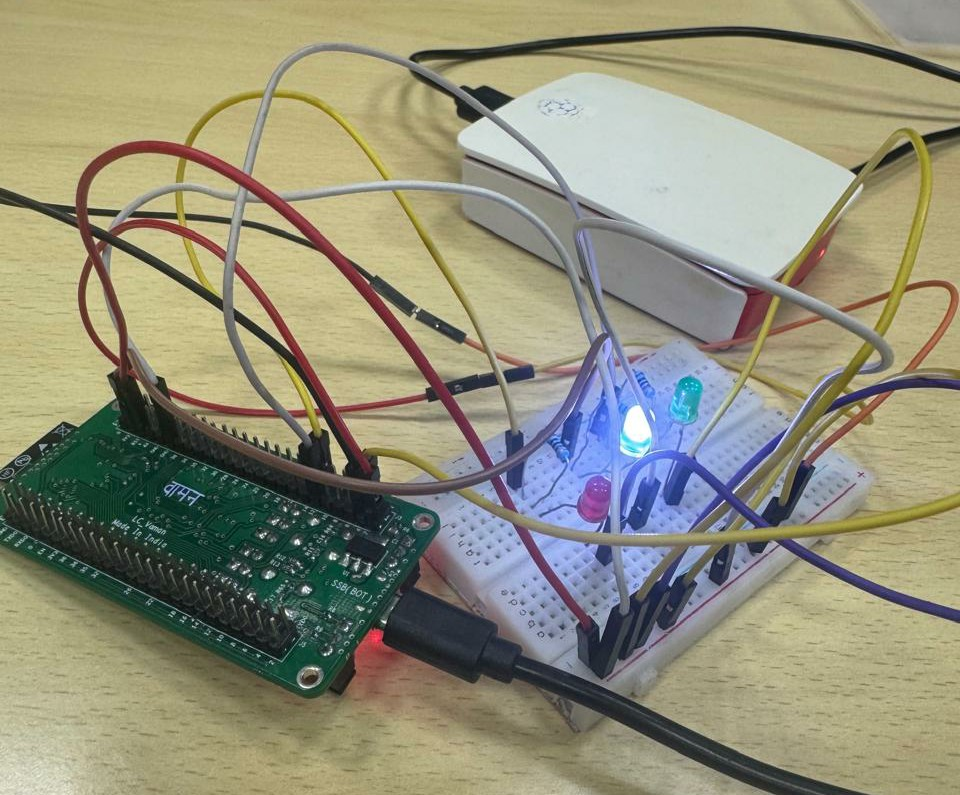
\includegraphics[width=0.35\textwidth]{/storage/emulated/0/FWC1/arm/IMG-20241111-WA0003~2.jpg   }
\caption{\label{fig:Gates}}
\end{figure}

\begin{table}[htbp]
\centering
\begin{tabular}{|c|c|c|c|c|} \hline
B & D & BD & $\overline{BD}$ & AB \\ \hline
0 & 0 & 1 OFF & ON & ON \\ \hline
0 & 1 & 1 OFF & OFF & ON \\ \hline
1 & 0 & 3 OFF & OFF & ON \\ \hline
1 & 1 & 20 ON & OFF & ON \\ \hline
\end{tabular}
\vspace{0.1cm}
\caption{\label{tab:widgets}}
\end{table}

\section{CONCLUSION}
This project demonstrated the practical application of Boolean algebra and digital logic using simple hardware components like LEDs and GPIO control. By successfully implementing the essential prime implicants $BD$, $\overline{BD}$, and $AB$, the project provided a clear visualization of logical functions in real-time hardware interaction. The setup can be extended to handle more complex Boolean functions or adapted for other hardware platforms, reinforcing key concepts in digital logic, hardware interfacing, and embedded systems programming.

\end{document}

